
\begin{comment}
%================================================================
\begin{frame}{From Data to Knowledge}
\framesubtitle{Activities: 12 laboratories involved, 18 teams, 64 registered researchers, about 20 participants per meeting}

Meetings topics (including 2 national and 1 international speakers):
\begin{itemize}
\item Information extraction from texts, ontologies
\item Modeling and processes
\item Knowledge and image analysis
\item Knowledge and reasoning
\item Multimedia content analysis
\end{itemize}

\end{frame}
\end{comment}

%================================================================
\begin{frame}{From Data to Knowledge}
\framesubtitle{Contact: Claire Nedellec (INRA) \& Chantal Reynaud (LRI)}
\vspace{-5mm}
{\color{blue} \contacturl{http://labex-digicosme.fr/GT+D2K}}

Activities: 12 laboratories involved, 18 teams, 64 registered researchers, about 20 participants per meeting
%
\begin{itemize}
  \small
  \item[$\rightarrow$] \emph{CS for modeling living organisms} $\rightarrow$ priority topic in the Life Sciences Department SGT5
  \item[$\rightarrow$] Issued a document included in the \emph{Life Sciences Department White Paper}

\item Led to ANR-DFG project GoASQ (ANR-DFG: LRI-LIMSI-TUD, 2015--2019): \emph{Generating and Answering Ontological Queries over Semi-structured Data}
\item Contribution to the B2SRI Strategic Research Institute application
  \begin{itemize}
  \item Systems Biology and Synthetic Biology for Research and Innovation (Life Sciences + CS)
  \end{itemize}
\item Two teams collaborate in H2020 E-Infra OpenMinTeD: Open Mining Infrastructure for Text and Data (2015--2018)
\item DigiCosme Invited Professor: Kevin B.\ Cohen (U.\ Colorado), text mining in biomedicine (3 months, 2016)
\end{itemize}
\end{frame}


%================================================================
\begin{frame}{Building a cartographic map of scientific communities (SciCoSense) }
%================================================================
  \framesubtitle{Contact: Philippe Caillou, LRI}
\vspace*{-1cm}
{\color{blue}
\contacturl{http://labex-digicosme.fr/GT+SciCoSense}}
  \begin{columns}
    \begin{column}{4cm}
      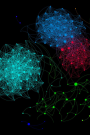
\includegraphics[width=\linewidth]{Images/scicosence-image.png}
    \end{column}
    \begin{column}{10cm}
      Representation and study of social networks:
      \begin{itemize}
      \item Study scientific communities
      \item based on traces of their activities
      \item to build indicators, maps and query tools
      \item about scientific production
      \end{itemize}
      \end{column}
  \end{columns}


\end{frame}

%================================================================
\begin{frame}{Deep Learning and Distributed Representations}
%================================================================
\framesubtitle{Contact: Alexandre Allauzen, LIMSI ; Emmanuelle Frenoux, LIMSI }
\vspace{-1cm}
{\color{blue} \contacturl{http://labex-digicosme.fr/GT+Reseaux+profonds}}
\begin{columns}
  \begin{column}{8cm}
    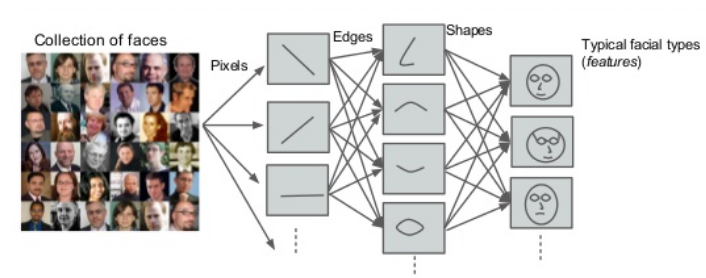
\includegraphics[width=\linewidth]{Images/dl.png}
  \end{column}
  \begin{column}{5cm}
    DataSense Task~3 (Machine learning)\\[2ex]
    
    \emph{Topic:}\\
    Deep neural networks and representation learning\\[2ex]
    
    \emph{Activities:}
    \begin{itemize}
    \item Journal club
    \item Cross-team presentations
    \item Invited seminars
    \end{itemize}
  \end{column}
  
\end{columns}
\vfill

  \emph{Participants:}\\
    LIMSI, CNRS (TLP, AMI) ---
    LRI, CNRS \& UPSud (TAO) ---
    U2IS, ENSTA ---
    LTCI, Télécom-ParisTech



\end{frame}


%================================================================
\begin{frame}{Prédiction et Analyse de données structurées et hétérogènes (PASADENA) }
%================================================================
\framesubtitle{Contact: 
Arthur Tenenhaus, Centrale-Supélec ; Maxime Sangnier, Télécom-ParisTech \&
Flora Jay, LRI}
\vspace{-5mm}
{\color{blue} \contacturl{ http://labex-digicosme.fr/GT+PASADENA}}

\begin{alertblock}{Objectives}
Developpement of statistical methods for complex data analysis: \textbf{heterogeneous}, \textbf{multimodal} and \textbf{structured} data:
\begin{itemize}
\item unsupervised analysis of correlations between modalities;
\item classification/regression from heterogeneous data;
\item structured prediction to fit a certain type of data from another;
\end{itemize}
\end{alertblock}


\begin{minipage}[c]{.7\linewidth}
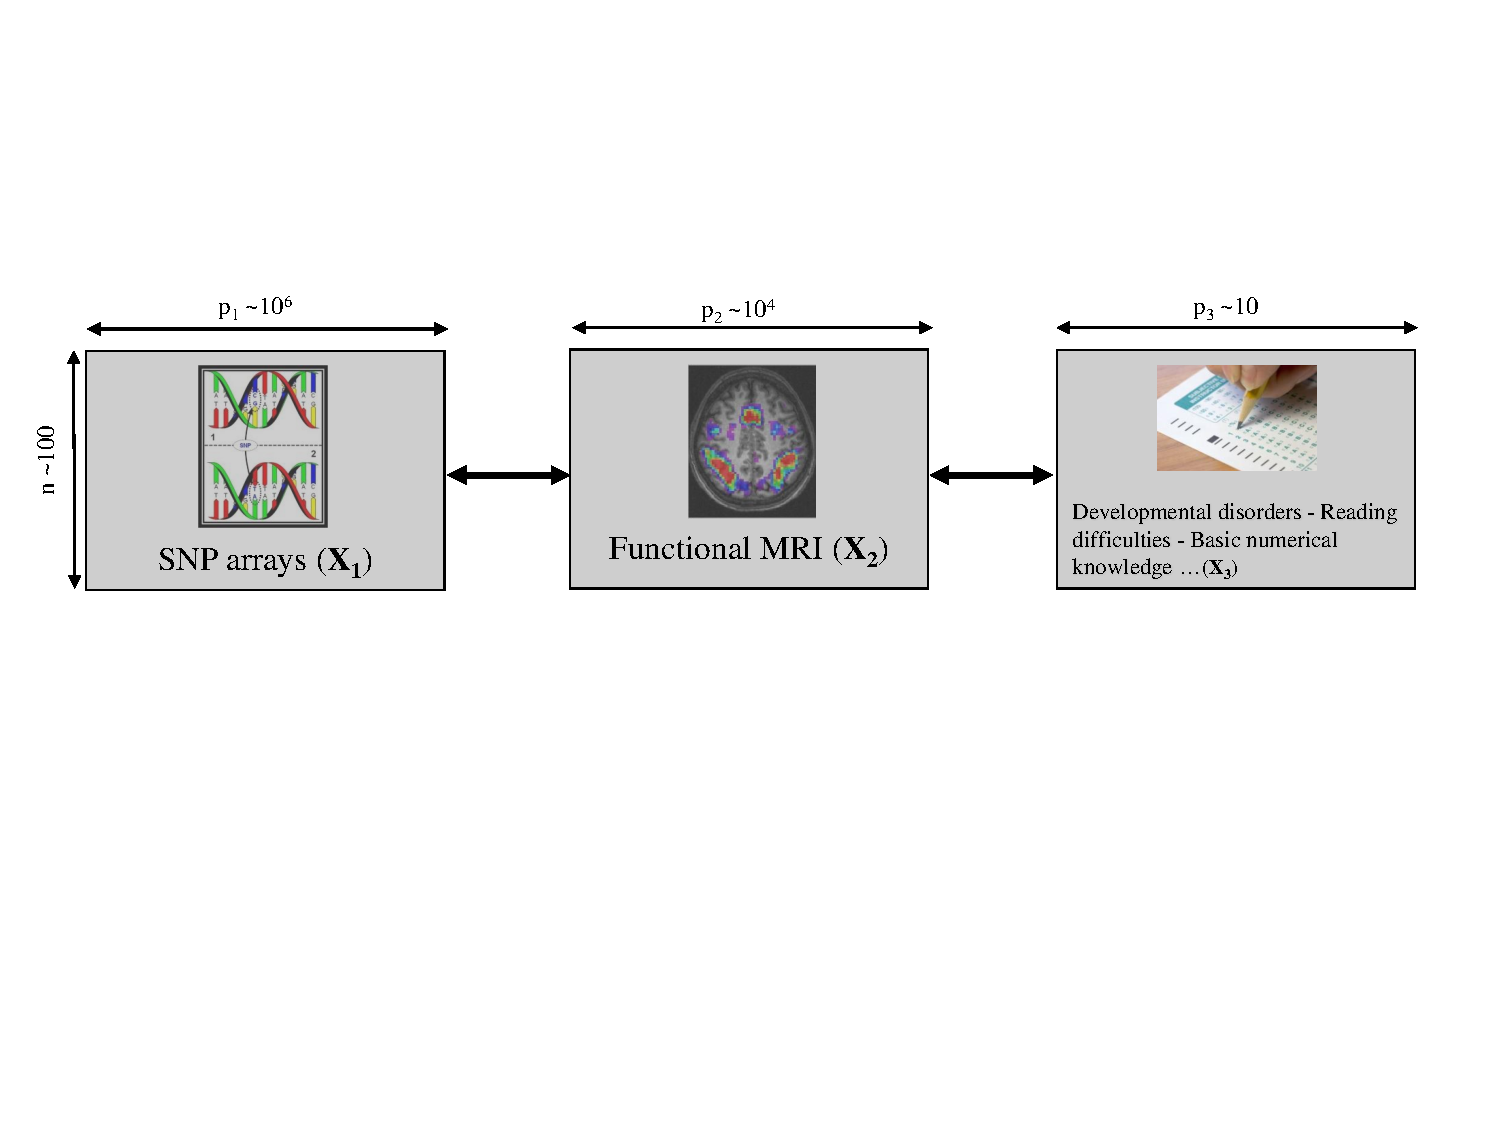
\includegraphics[trim = 0mm 90mm 0mm 50mm, clip, width=\linewidth]{Images/pasadena_poster_I.pdf}
\end{minipage}\hfill
\begin{minipage}[c]{.28\linewidth}
Multibloc study in imaging genetics.
\end{minipage}


\end{frame}



%================================================================
\begin{frame}{Human-Robot Interaction}
%================================================================
\framesubtitle{Contact: Laurence Devillers \& Jean-Calude Martin (LIMSI-CNRS) }
{\color{blue} \contacturl{http://labex-digicosme.fr/GT+Interaction}}

\begin{minipage}[c]{.35\linewidth}

\includegraphics[width=\linewidth]{Images/hr1.png}
\end{minipage} 
\hfill
\begin{minipage}[c]{.64\linewidth}
Objectives
\begin{itemize} 
\item Create a community on interactive robotics; verbal/non-verbal/physical Human-robot interactions 
\item Group specialists beyond robotics: modeling and interaction, big data, psychology, social and cognitive sciences, ergonomy and  usage, ethics.
\end{itemize}
 Members : LIMSI, ENSTA, CEA, Télécom SudParis, Télécom ParisTech, Télécom Ecole de Management, Université Paris-Sud, UVSQ, Université d’Evry, CERDI
\end{minipage}


\end{frame}


%================================================================
\begin{frame}{ERVEN : Extraction, Représentation et Visualisation de connaissance pour
l'Enseignement Numérique}
\framesubtitle{Contact: Anne-Laure Ligizat}
{\color{blue} \contacturl{https://digicosme.lri.fr/tiki-index.php?page=GT+ERVEN}}
\begin{columns}
  \begin{column}{7cm}
    \hspace*{-1cm}
    \begin{itemize}
    \item Équipes du LIMSI :
      \begin{itemize}
      \item
        Équipe ILES (Brigitte Grau, Gabriel Illouz, Anne-Laure Ligozat)
      \item
        Équipe AMI (Frédéric Vernier)
      \item
        Équipe TLP (Alexandre Allauzen) 
      \end{itemize}
    \item Équipes du LRI : 
      \begin{itemize}
      \item LaHDAK: Philippe Dague,
        Yue Ma, Brigitte Safar, Fatiha Saïs 
      \item MODHEL:Yolaine Bourda, Fabrice Popineau
      \end{itemize}
    \item SAMOVAR, Telecom SudParis :
      Amel Bouzeghoub 
    \end{itemize}
  \end{column}
  \begin{column}{6cm}
    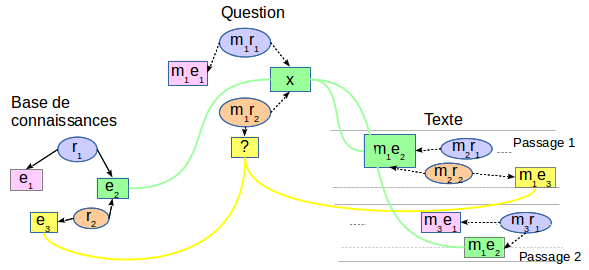
\includegraphics[width=6cm]{Images/education.png}
  \end{column}
\end{columns}
\end{frame}


\begin{frame}{E-santé : Internet des Objets and E-santé -- 2017 / 2019}
\framesubtitle{Contact : Mehdi Ammi}
%
\vspace{-1cm}
{\color{blue} \contacturl{https://digicosme.lri.fr/tiki-index.php?page=GT+Internet+des+objets+et+E-sante}}
%
%
\begin{columns}
  \begin{column}{6cm}
    \begin{itemize}
    \item étude, conception et évaluation des services e-santé
    \item traitement des données
    \item technologie
    \item éthique
    \end{itemize}
  \end{column}
  %
  \begin{column}{7cm}
    \begin{itemize}
    \item Laboratoires \textit{TIC}: LIMSI( AMI, CPU, ILES, TLP),
      ENSTA ParisTech, CIAMS, Telecom SudParis, CEA-LIST, LRI
    \item Laboratoire \textit{Santé} End-icap Fondation Helene -
      Poidatz Handiresp Hôpital Bicêtre
    \item \textit{Associations et pôles}: RevesDiab France eHealthTech
      Systematic Capdigital OpticsValley Fedev (SFR)
    \end{itemize}
  \end{column}
\end{columns}
\end{frame}


\begin{frame}{ TAL \& SEM : Traitement sémantique des données textuelles – 2017 / 2018}
\framesubtitle{Contact : Brigitte Grau, LIMSI}
\vspace{-1cm}
{\color{blue} \contacturl{https://digicosme.lri.fr/tiki-index.php?page=GT+TAL+et+SEM}}
\\
Implication textuelle, paraphrase, désambiguisation sémantique

\begin{columns}
\begin{column}{8cm}
\begin{itemize}
\item \textbf{Timothy Miller}: Boston Children's Hospital, Introduction to sequence models for Natural Language Processing
\item \textbf{Brigitte Grau}: LIMSI, De la recherche de réponses à des questions à la compréhension ciblée de textes
\item \textbf{Olivier Ferret}: Apprentissage de connaissances sémantiques : adaptation de plongements lexicaux (words embeddings) à des connaissances externes
\end{itemize}
\end{column}
\begin{column}{5cm}
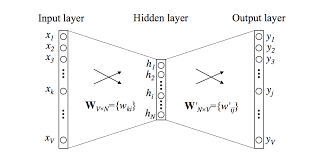
\includegraphics[width=5cm]{Images/language.png}
\end{column}
\end{columns}
\end{frame}

\vspace{-1cm}
\begin{frame}{SDT : Sécurité des Données Textuelles – 2016 / 2017}
\framesubtitle{Contact : Cyril Grouin, LIMSI}
{\color{blue} \contacturl{https://digicosme.lri.fr/tiki-index.php?page=GT_SDT}}

Common group with Scilex
\begin{columns}
\begin{column}{8cm}
\begin{itemize}
\item LIMSI : équipe ILES (Cyril Grouin (CNRS), Thomas Lavergne (Université Paris-Sud), Aurélie Névéol (CNRS), Pierre Zweigenbaum (CNRS)
\item INRIA-LIX : équipe COMETE (Catuscia Palamidessi, Kostantinos Chatzikokolakis)
\item CEA-LIST, équipe LVIC (Olivier Ferret, Gaël de Chalendar)
\end{itemize}
\end{column}
\begin{column}{5cm}
\begin{itemize}
\item
Anonymisation et risques de réidentification
\item
Protection des données dans les modèles
\item
Optimisation de la confidentialité différentielle
\end{itemize}
\end{column}
\end{columns}
\end{frame}

\begin{frame}{SSSL : Séquential Structured Statistical Learning – 2015 / 2017}
\framesubtitle{Contact : Oldaric Maillard, LRI}
\contacturl{https://sites.google.com/site/groupedetravailsssl/home}
\begin{columns}
\begin{column}{10cm}
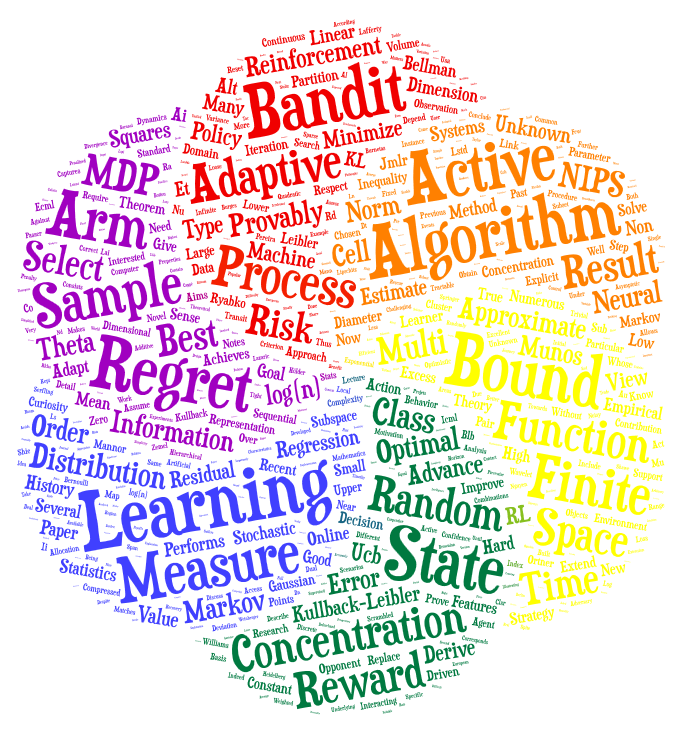
\includegraphics[width=6cm]{Images/Cloud-13.png}
\end{column}
\end{columns}
\end{frame}
